\documentclass{article}

\usepackage[portuguese]{babel}

\usepackage{amsmath, amssymb}
\usepackage{graphicx}
\usepackage[colorlinks=true, allcolors=blue]{hyperref}

\usepackage[section]{placeins}

\title{Lista 02}
\author{Vinícius de Oliveira Peixoto Rodrigues (245294)}
\date{Setembro de 2022}

\begin{document}
\maketitle

\section*{Questão 1}

A propriedade pode ser usada para diminuir o número de tentativas necessárias de se encontrar a chave por força bruta (testando todas as chaves possíveis). Se $K$ é a chave original, vamos testar os valores de $E_k(P_1)$ para todas as chaves $k$ possíveis. A propriedade do complemento nos dá duas informações importantes:

\begin{itemize}
    \item se $E_k(P_1) = C_1 \Leftrightarrow K = k$
    \item se $E_k(P_1) = C_2' \Leftrightarrow K = k'$, visto que $E_K(P_1') = C_2 \Rightarrow E_{K'}(P_1) = C_2'$
\end{itemize}

(o $\Leftrightarrow$ vem do fato de que é muito pouco provável que dois plaintexts produzam a mesma saída). Essa é uma vantagem muito poderosa, visto que permite, com apenas um cálculo de ciphertext $E_k(P_1)$, eliminar duas chaves por vez, reduzindo pela metade o esforço para encontrar a chave por força bruta.

\section*{Questão 2}

\subsection*{Item (a)}

O 2DES é vulnerável a ataques meet-in-the-middle. Sejam $k_1$, $k_2$ as duas chaves usadas; a ideia é encriptar uma entrada $P$ usando a chave $k_1$, e em seguida encriptar o resultado usando a chave $k_2$:

\begin{equation*}
    P \rightarrow E_{k_1}(P) \rightarrow E_{k_2}(E_{k_1}(P)) \rightarrow C
\end{equation*}

A ideia do meet-in-the-middle é calcular os pares P-C para todas as chaves possíveis usando a entrada $P$, e guardá-los em uma lookup table:

\begin{gather*}
    \underbrace{E_k(P)}_{\text{all possible $k$}} = C_k \\
    \text{table}(C_k) \mapsto k
\end{gather*}

e, em seguida, para cada chave $k$, decifrar a saída C, e procurar um match com a tabela de busca:

\begin{gather*}
    \text{table}(\underbrace{D_k(C)}_{\text{all possible $k$}}) == k ? \\
\end{gather*}

Isso faz com que sejam necessários somente $2 \cdot 2^{56}$ cálculos do DES para se quebrar o 2DES. Por essa razão se escolheu usar o 3DES:

\begin{gather*}
    P \rightarrow E_{k_1}(P) \rightarrow E_{k_2}(E_{k_1}(P)) \rightarrow 
        E_{k_3}(E_{k_2}(E_{k_1}(P))) \rightarrow C
\end{gather*}

visto que a abordagem do meet-in-the-middle aqui forçaria o invasor a calcular todas as possibilidades de combinação de chaves $k_1$ e $k_2$, resultando em $2^{112}$ operações para montar a lookup table, mais $2^{56}$ operações para testar todas as possibilidades de $k_3$.

\subsection*{Item (b)}

Mesmo fazendo $k_1 = k_3$, o atacante ainda teria que montar uma tabela com todas as $2^{112}$ combinações possíveis de $(k_1, k_2)$, o que ainda assim custaria $2^{112}$ operações.

\section*{Questão 3}

O módulo de Feistel é um procedimento iterativo com vários rounds (normalmente 16) que funciona como caso particular de uma estrutura proposta por Shannon, chamada substitution-permutation network.

No algoritmo, é recebida uma entrada de $2w$ bits, que vai ser modificada repetidamente. É também recebida uma chave $K$, e a partir dela são geradas subchaves $\{K_1, K_2, ... K_n\}$, tantas quanto o número de rounds. A cada round, o bloco em duas partes: $LE_k$ e $RE_k$ (cada uma de comprimento $w$), e o fluxo básico de modificação do bloco em cada round é:

\begin{itemize}
    \item $LE_{i+1} = RE_i$
    \item $RE_{i+1} = LE_i \oplus F(RE_i, K_i)$
\end{itemize}

onde $F(RE_k, K_i)$ é a chamada função de Feistel (função F), cujo objetivo é aumentar a confusão da cifra.

No DES, há 16 rounds e a entrada tem 64 bits, enquanto a chave tem 56 (o algoritmo recebe 64, mas 8 são de verificação de paridade).

Cada subchave tem 48 bits e é gerada a partir do seguinte processo:

\begin{itemize}
    \item Escolher 56 dentres os 64 bits da chave (normalmente descarta-se ou usa-se como parity check os bits múltiplos de 8, e em seguida embaralha-se os bits restantes): \textit{Permuted choice 1 (PC-1)}
    \item Separa-se a chave em duas metades de 28 bits
    \item Fazem-se 16 rounds onde as duas metades sofrem separadamente um left-shift de 1 ou 2 bits, e em seguida são selecionados 48 bits para a geração da subchave: \textit{Permuted choice 2 (PC-2)}
\end{itemize}

Já a função $F(RE_i, K_i)$ do DES recebe um bloco de tamanho 32 bits e uma chave de tamanho 48 bits, e tem o seguinte fluxo:

\begin{itemize}
    \item Expansão: o bloco de entrada é expandido para 48-bits usando a permutação de expansão (\textit{E-expansion}), duplicando metade dos bits
    \item Mistura com a chave: é feito um XOR do resultado com a subchave do round
    \item Substituição: o bloco é dividido em 8 sub-blocos de 6 bits cada, e passa por uma transformação (\textit{S-boxes}) que transforma os 6 bits de entrada em 4 bits de saída de forma não-linear (isso é responsável pela segurança da cifra)
    \item Permutação: os 32 bits de saída das \textit{S-boxes} são embaralhados de acordo com uma permutação fixa (\textit{P-box}).
\end{itemize}

Vale notar que na função F acima, as \textit{S-boxes} implementam a confusão, enquanto a \textit{P-box} e a \textit{E-expansion} implemantam a difusão.


\section*{Questão 4}

As subchaves começariam a se repetir. Isso se deve ao fato de que na etapa de left-shifts da geração de subchaves, existe uma tabela (\textit{bits rotation table}) que define se cada sub-bloco de 28 bits (correspondente a uma metade do estado atual, de 56 bits, do gerador de subchaves), vai sofrer left-shift de 1 ou 2 posições:

\newpage
\FloatBarrier
\begin{figure}[!ht]
    \begin{center}
        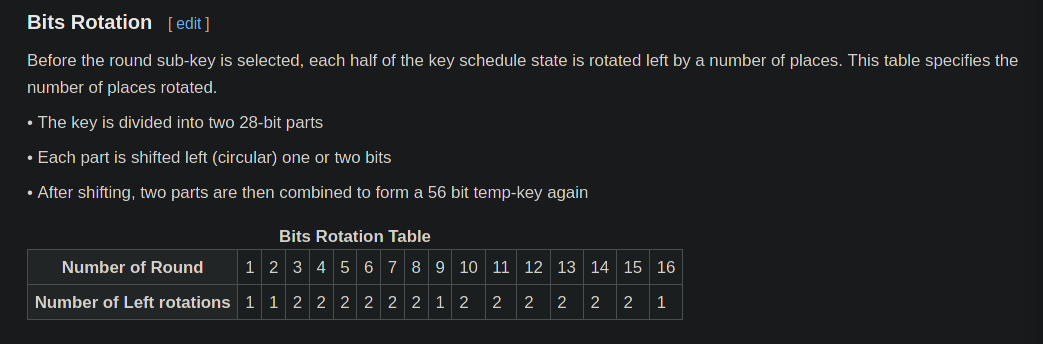
\includegraphics[width=\textwidth]{images/bit-rotation-table.png}
        \caption{Fonte: \url{https://en.wikipedia.org/wiki/DES_supplementary_material}}
    \end{center}
\end{figure} 

A soma do número de bits a rotacionar o estado do gerador é 28, de modo que após os 16 rounds, o estado de gerador volta a ser igual ao inicial, e todas as subchaves geradas posteriormente vão ser repetições cíclicas das dos primeiros 16 rounds.

\section*{Questão 5}

O nome criptanálise diferencial vem de uma observação a respeito de conjuntos de plaintext com \textbf{diferença} constante, onde a diferença é definida simplesmente como $P \oplus P^* = P'$.

A ideia básica é que, para uma chave fixa, a distribuição de pares plaintext-chiphertext $(P, C)$ é em geral uniforme, mas quando se escolhem plaintexts $(P, P^*)$ com \textbf{diferença} constante, a distribuição da diferença entre os ciphertexts $(C, C^*)$ \textbf{deixa de ser uniforme}.

Em um DES hipotético de 1 round, isso permite encontrar padrões estatísticos entre a entrada/saída das \textit{S-boxes} do DES, o que por sua vez permite encontrar os candidatos mais prováveis de subchaves para o round. Os desenvolvedores do algoritmo estavam cientes disso e essa é a razão pela qual o DES possui muitos rounds (quantos mais rounds, mais difícil fazer esse tipo de análise). Contudo, mudanças pequenas na estrutura do DES podem gerar resultados catastróficos que aumentam a vulnerabilidade da cifra a esse tipo de ataque.

\section*{Questão 6}

\begin{itemize}
    \item Add round key: nesta etapa, cada byte do estado é combinado com um byte da chave do round por meio de um XOR
    \item Substitute bytes: é feita uma substituição não-linear de cada byte do estado (\textit{S-boxes}), de forma semelhante ao DES
    \item Shift rows
    \item Mix columns
\end{itemize}

\end{document}
